\section{Durchführung}
\label{sec:Durchführung}
Zur Durchführung des Versuchs ist ein Aufbau notwendig, der in \autoref{fig:Aufbau_Skizze} dargestellt ist.
Die Wärmepumpe ist in zwei Teilbereiche gegliedert. In den beiden Bereichen befindet sich je ein thermisch isoliertes Gefäß (Reservoir), ein Digital-Thermometer und 
ein Manometer. Die Reservoire werden mit Wasser befüllt. Im \dq kalten\dq\: Bereich (links) wird die Temperatur $T_2$ des Wassers und der Druck $p_a$ im Inneren der Rohrleitung 
gemessen. Im \dq warmen\dq\: Bereich bezeichnen $T_1$ und $p_b$ die Temperatur des Reservoirs und den Druck in der Leitung. Das Drosselventil zwischen den Teilbereichen regelt 
die Durchflussmenge des Transportgases anhand der Temperaturdifferenz. Das verwendete Gas ist Dichlordifluormethan ($\text{Cl}_2\text{F}_2\text{C}$). Der Kompressor dient zur Erzeugung des 
Druckunterschieds in den beiden Teilbereichen. Seine momentane Leistungsaufnahme kann am Leistungsmesser (Wattmeter) abgelesen werden. In den isolierten Gefäßen ist ein Rührmotor 
installiert, der eine Vermischung des Wassers gewährleistet, damit eine möglichst homogene Temperaturverteilung in diesem gegeben ist. Ein \dq Reiniger\dq \: und eine 
Steuerungsvorrichtung sorgen dafür, dass das verflüssigte Transportmedium von Gasresten getrennt wird und keine Flüssigkeit in den Kompressor gelangt. Diese Apparaturen sind 
nicht in \autoref{fig:Aufbau_Skizze} zu sehen. In \autoref{fig:Aufbau_real} sind die beschriebenen Geräte und deren Anordnung im realen Versuchsaufbau zu sehen.

\begin{figure}
    \centering
    \caption{Schematische Darstellung des Versuchaufbaus. \cite{v206}}
    \label{fig:Aufbau_Skizze}
    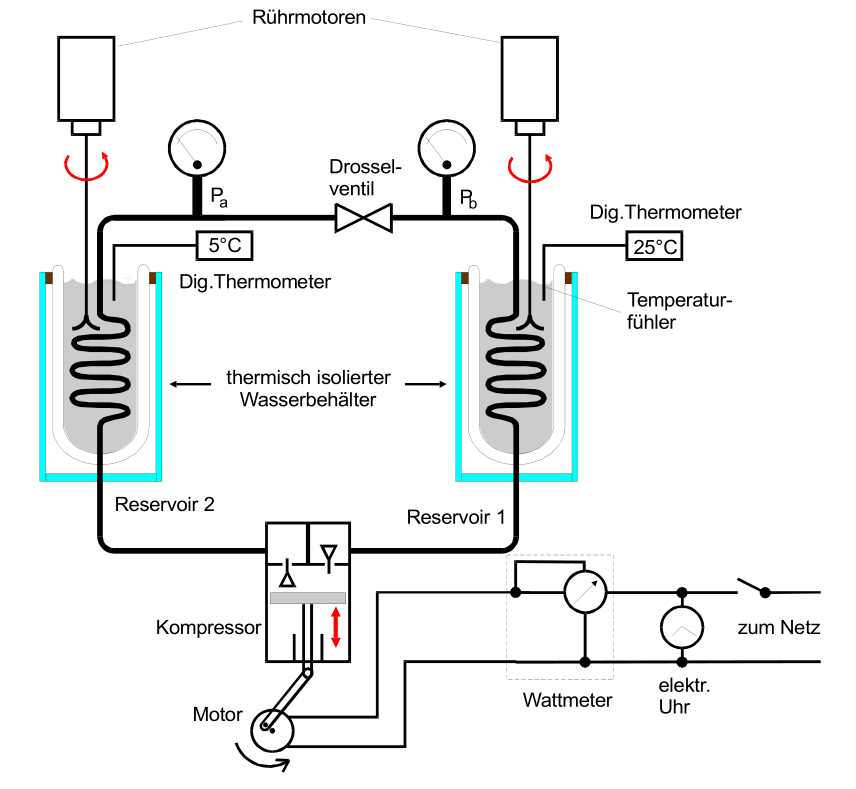
\includegraphics[width=.5\textwidth]{content/Aufbau_Skizze.png}
\end{figure}

\begin{figure}
    \centering
    \caption{Bild des konkreten Aufbaus.}
    \label{fig:Aufbau_real}
    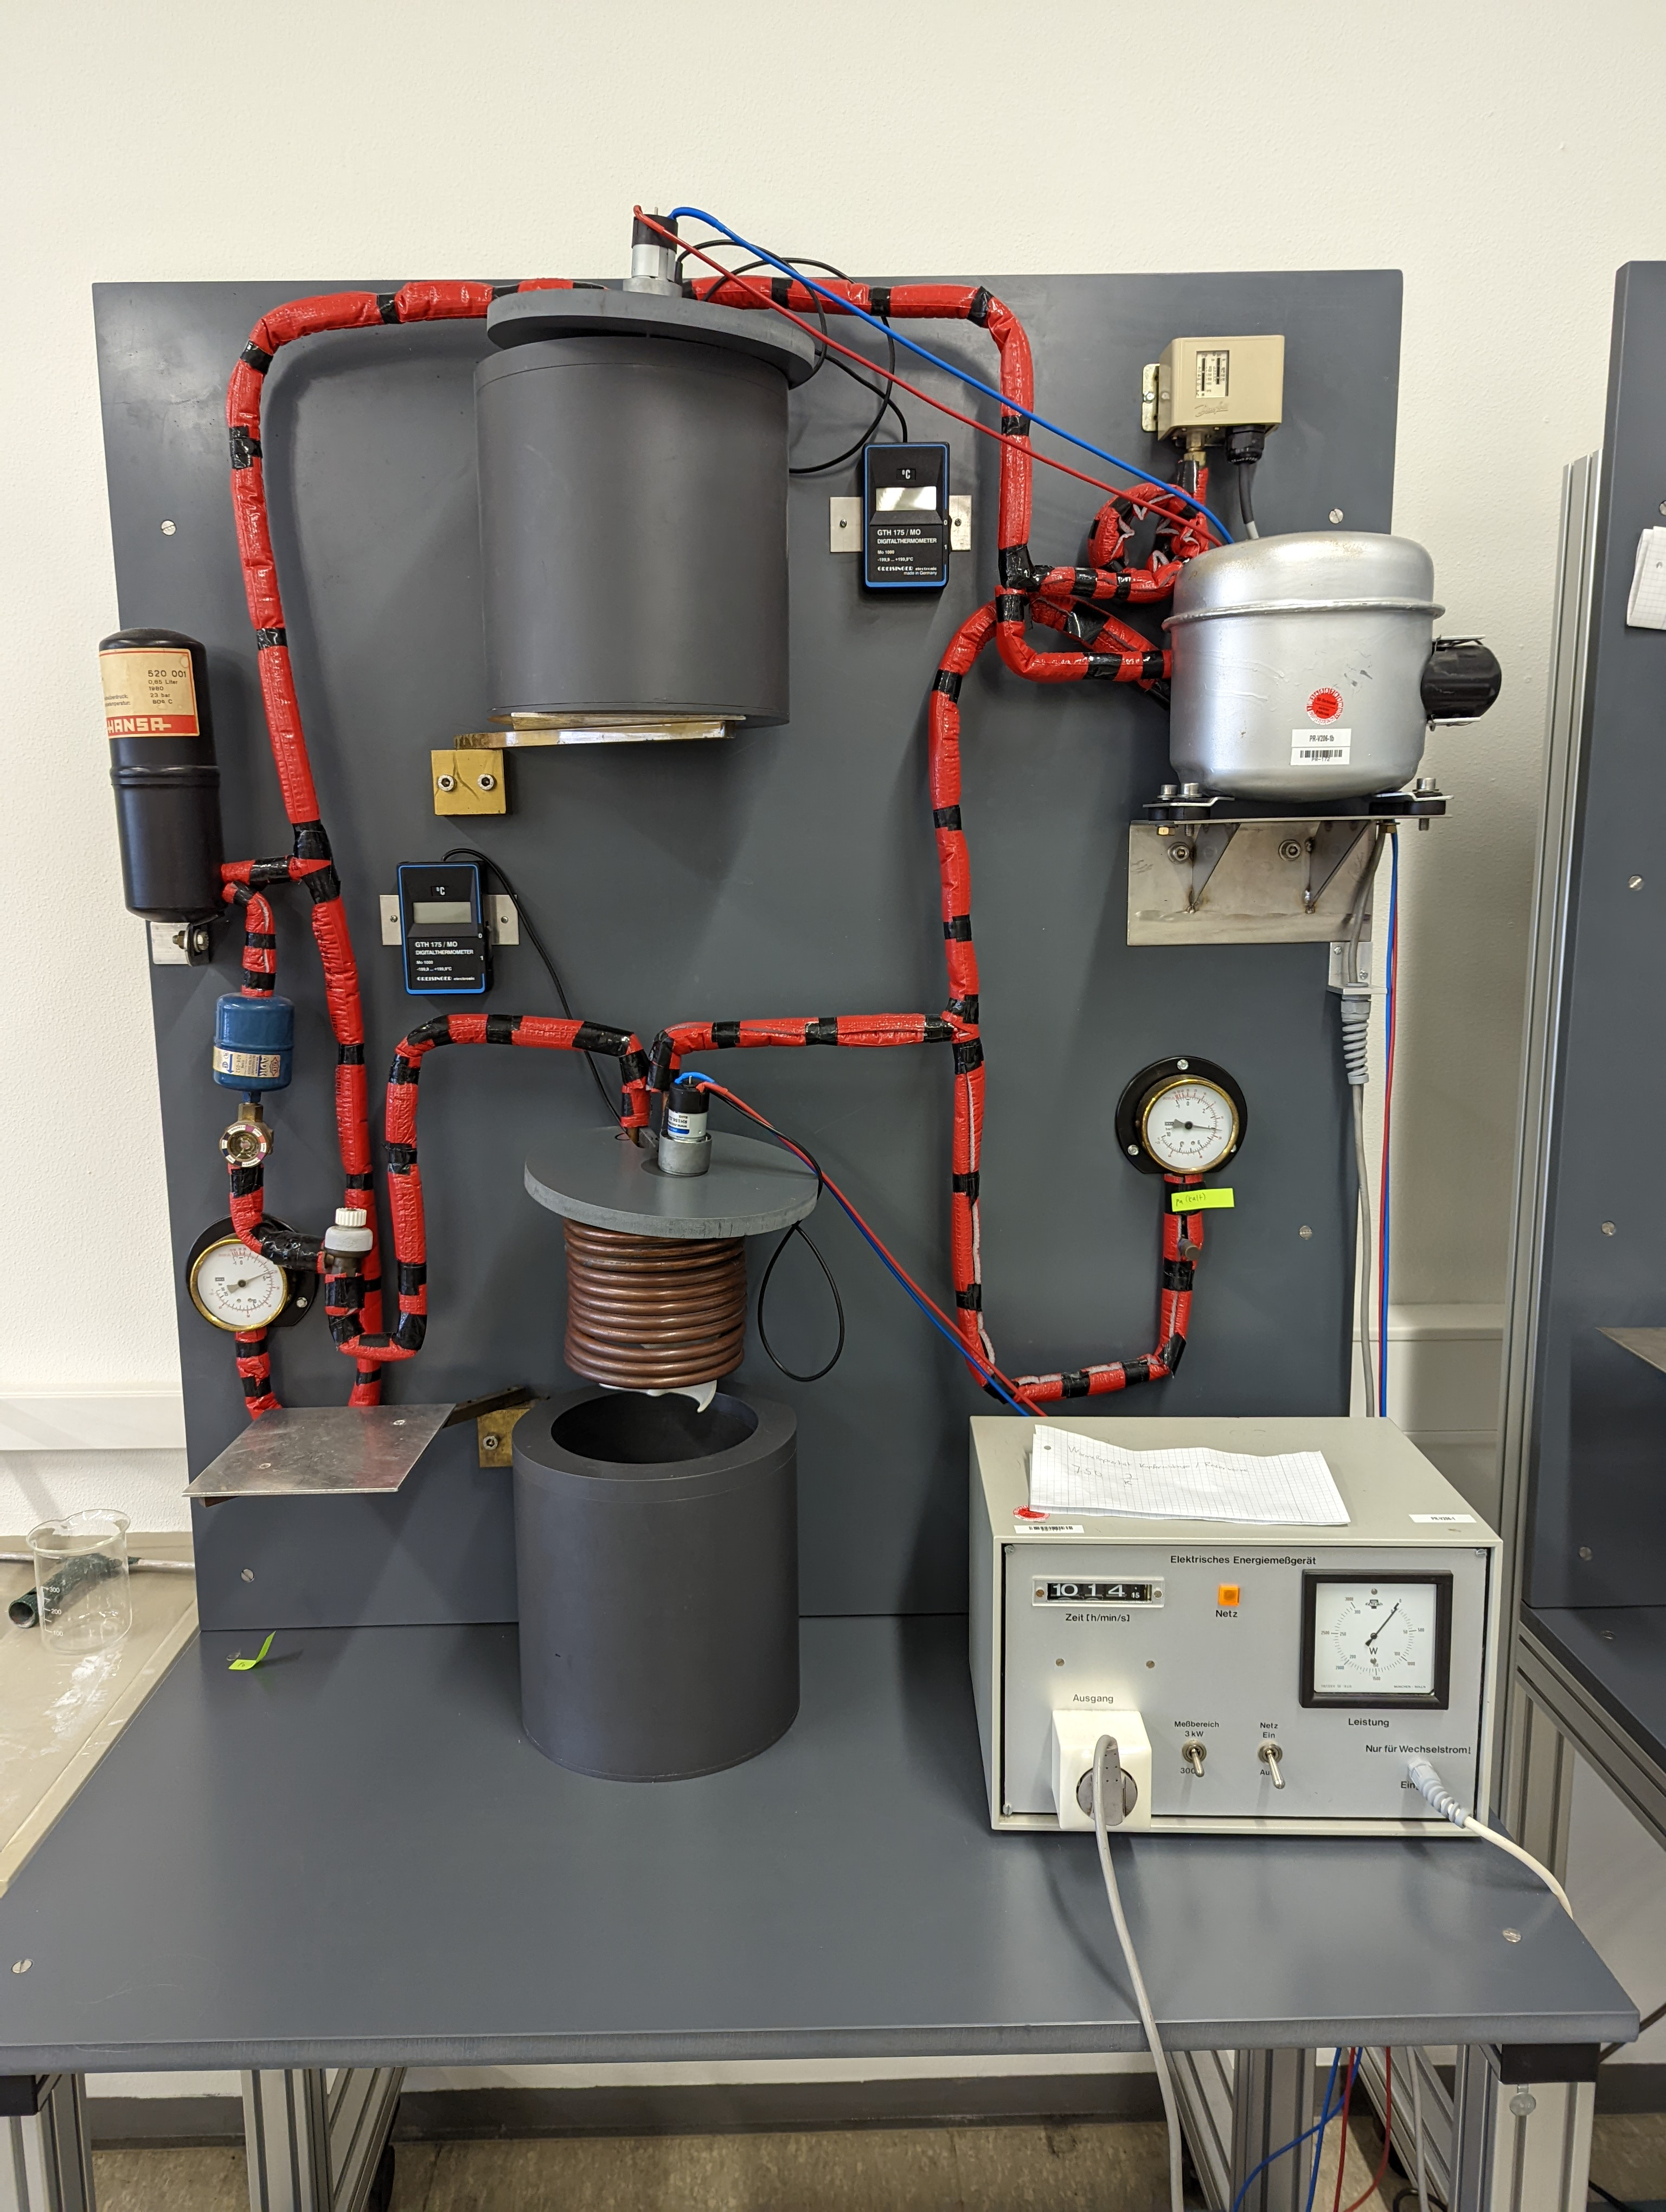
\includegraphics[width=.4\textwidth]{content/Gesamtbild.jpg}
\end{figure}

Bevor der Versuch durchgeführt werden kann, müssen je 3 Liter Wasser in die Gefäße gefüllt werden, die mit einem Messkolben abgemessen werden.
Das eingefüllte Wasser hat Raumtemperatur also etwa $21,7 \unit{\degreeCelsius}$.
Anschließend werden die Rührmotoren eingeschaltet. Sobald nun der Strom am Wattmeter eingeschaltet wird beginnt die Messung. Alle 60 Sekunden werden
die Temperaturen $T_1$ und $T_2$, die Drücke $p_a$ und $p_b$, sowie die Leistung des Kompressors notiert. Bei den Drücken ist darauf zu achten, dass die analogen Druckmesser
nur den Relativdruck zur Atmosphäre anzeigen, weshalb zu den Messwerten $1 \unit{\bar}$ addiert werden muss. Das Ablesen der fünf Messwerte sollte möglichst zeitgleich beziehungsweise
in einem kurzen Zeitraum erfolgen.

Im Verlauf der Messung steigt die Temperatur im Reservoir 2, während Die des zweiten Reservoirs abfällt. Ist ein Wert von $50 \unit{\degreeCelsius}$
im warmen Reservoir erreicht, wird der Kompressor ausgeschaltet und die Messung beendet. Sollte vorher $0 \unit{\degreeCelsius}$ im kalten Reservoir unterschritten werden, muss die
Messung ebenfalls abgebrochen werden, da sonst Teile des Aufbaus gefrieren können.